\documentclass{article}

\usepackage{xcolor}
\usepackage[margin=0.5in]{geometry} 
\usepackage{graphicx}

\graphicspath{{images/}}

\begin{document}

\newpage
\newgeometry{margin=1.5in}
\section*{Abstract}   % titolo temporaneo da modificare
In today's rapidly evolving business landscape, the importance of advanced technological tools becomes increasingly evident. The current market is characterized by swift and unpredictable changes, fueled by a myriad of factors such as technological advancement and the complex global geopolitical landscape. In this already intricate scenario, economic fluctuations and the growing expectations of consumers demand significant efforts from companies to remain competitive 
and meet the evolving needs of the market. All things considered, many uncertainties arise:

% NON E' UNA LISTA! -> mettere una lista sarebbe un errore (e' un flusso di domande, NON un elenco comprensivo!)
% sebbene quindi sbagliato penso pero' sia graficamente piu' piacevole, faro' la lista comunque
\begin{itemize}
    \item How will the market change as these models become more efficient and effective?
    \item What must companies do to remain competitive in the evolving market?
    \item What opportunities exist today for companies to harness these technologies?
\end{itemize}
These were the uncertainties and presumptions of the present-day world.\\
% vvvvv riga vuota per enfatizzare l'ultima frase
\\
What follows our response.
\\
\\
\\
\\
\\

\section*{MindMerge}
\pagebreak
\restoregeometry

\section{SWAT Analysis}
\subsection{Quick recap}
The development of software must incorporate a comprehensive evaluation of the economic environment in which it will operate.
Within this framework, the SWOT analysis emerges as a vital instrument for gaining a profound understanding of the surrounding landscape, enabling the formulation of a cohesive strategy to tackle challenges and leverage opportunities.

\begin{figure}[h]
  \centering
  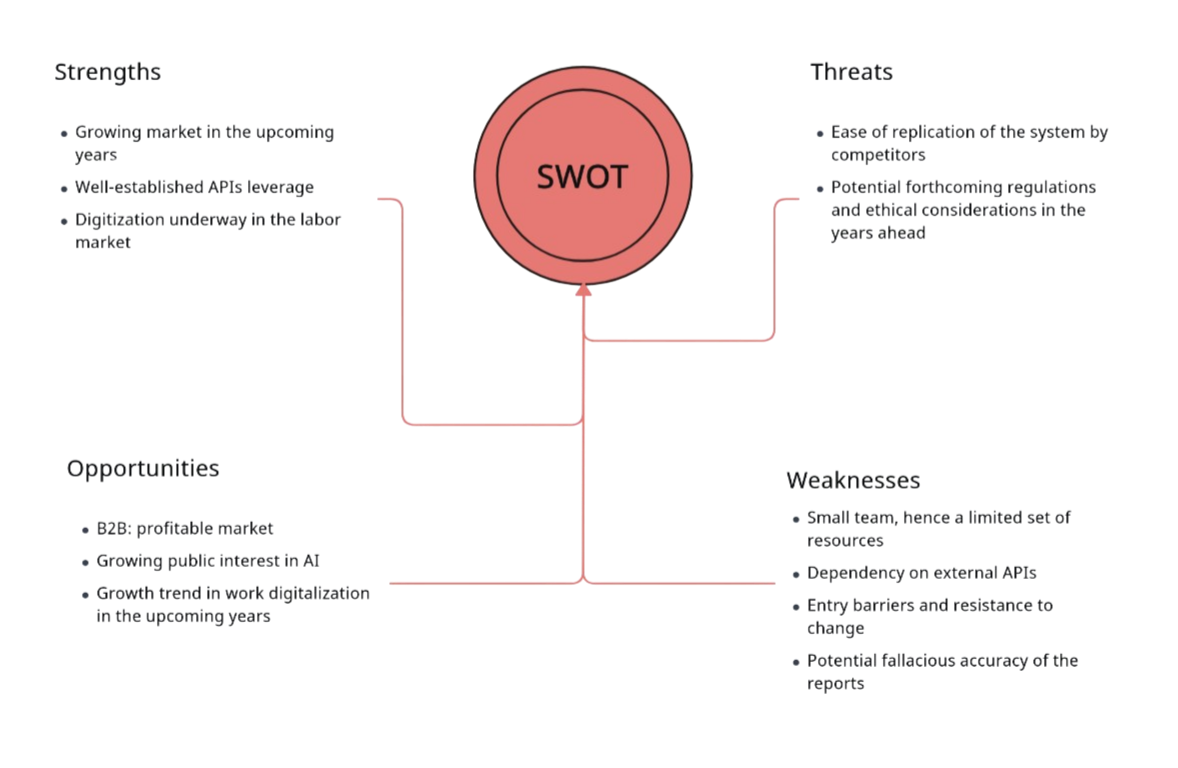
\includegraphics[width=0.95\textwidth]{swat_cropped.png}
  \caption{\small SWOT Analysis Diagram: visual representation of the Strengths, Weaknesses, Opportunities, and Threats associated with our software project}
\end{figure}
\end{document}
